\documentclass[11pt]{amsart}
\usepackage{geometry}                % See geometry.pdf to learn the layout options. There are lots.
\geometry{letterpaper}                   % ... or a4paper or a5paper or ... 
%\geometry{landscape}                % Activate for for rotated page geometry
%\usepackage[parfill]{parskip}    % Activate to begin paragraphs with an empty line rather than an indent
\usepackage{graphicx}
\usepackage{amssymb}
\usepackage{epstopdf}
\usepackage[usenames,dvipsnames]{color}
\usepackage{fancyvrb}
\usepackage{listings}
\usepackage{booktabs,footmisc}
\usepackage{hyperref}
\usepackage[all]{hypcap}

\usepackage{topcapt}


 
% include the lines below to use a nicer fixed-width font than the default one
 
\lstset{fancyvrb=true}
\lstset{
	basicstyle=\small\tt,
	identifierstyle=,
	commentstyle=\color{Bittersweet},
	stringstyle=\color{red},
	showstringspaces=false,
	tabsize=3,
	numbers=left,
	captionpos=b,
	xleftmargin=2em
%	numberstyle=\tiny
	%stepnumber=4
	}
\DeclareGraphicsRule{.tif}{png}{.png}{`convert #1 `dirname #1`/`basename #1 .tif`.png}

\title{Repast Statecharts Guide}
\author{Jonathan Ozik, Nick Collier - Repast Development Team}
\date{\today}                                           % Activate to display a given date or no date

\begin{document} 
\maketitle
\setcounter{section}{-1}

\section{Before we Get Started}
Before we can do anything with Repast Simphony, we need to make sure that we have a proper installation of Repast Simphony 2.1. Instructions on downloading and installing Repast Simphony on various platforms can be found on the \href{http://repast.sourceforge.net/download.html}{Repast website}\footnote{http://repast.sourceforge.net/download.html}. Repast Simphony 2.1 requires Java 7. Java 7 can be found at the \href{http://www.oracle.com/technetwork/java/javase/downloads/index.html}{Java Standard Edition Downloads page}\footnote{http://www.oracle.com/technetwork/java/javase/downloads/index.html}.

\section{Getting Started with Statecharts}

Agent states and transitions between states are an important abstraction in agent-based modeling. While it is possible for Repast Simphony users to create their own implementation of state-based agent behaviors (e.g., by adapting the State pattern in Gamma et al. 1994\footnote{Gamma, E., R. Helm, R. Johnson, and J. M. Vlissides. Design Patterns: Elements of Reusable Object-Oriented Software. illustrated ed. Addison-Wesley Professional, 1994.}) and even agent state visualizations, the effort involved in doing so is usually prohibitive. By integrating an agent statecharts framework into Repast Simphony, we made it easy for users of all levels to take advantage of this important modeling paradigm. Statecharts are visual representations of states and the transitions between those states\footnote{Statecharts were first proposed by Harel in Harel, D., 1987. Statecharts: A visual formalism for complex systems. Sci. Comput. Program., 8(3), pp.231-274.}. Statecharts can be very effective in visually capturing the logic within agents and quickly conveying the underlying dynamics of complex models.

Figure~\ref{fig:statechartExample} shows a simple example of a statechart created with the Repast Simphony statecharts framework. The logic embedded in the diagram is mapped directly to the execution logic of an agent-based model. The benefits of the Repast Simphony statecharts framework include: improved clarity of a model's logic for model design, improved turnaround times for developing complex state based agent models, and the ability to convey in a compelling manner the internal state of agents as a simulation evolves to both experienced agent-modelers and to non-modelers alike. In the rest of this guide we will present the Repast Simphony statecharts framework.

\begin{figure}
\begin{center}
\vspace{.2in}
\centerline {
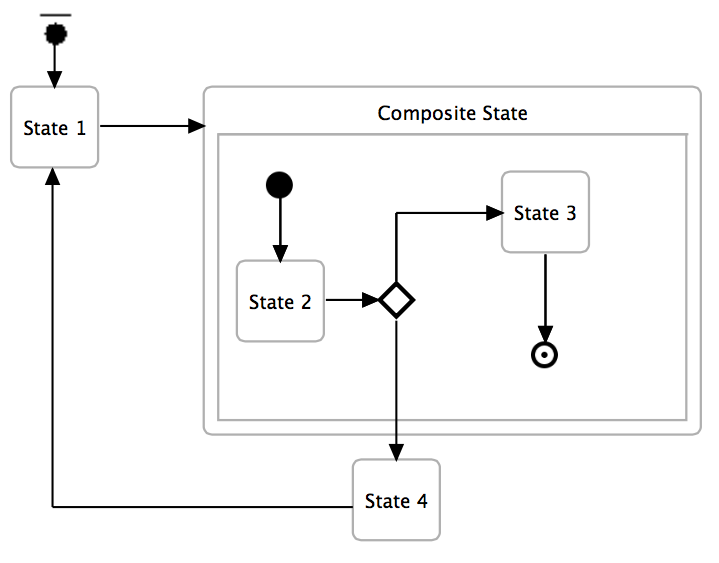
\includegraphics[width=5in]{StatechartsImages/StatechartExample.png}
}
\caption{An example statechart created with the Repast Simphony visual statecharts editor.}
\label{fig:statechartExample}
\end{center}
\end{figure}

\subsection{Adding Statecharts}
A statechart can be added to any Java, Groovy or ReLogo class. Right-clicking the class of interest and selecting New $\rightarrow$ Statechart Diagram (Figure~\ref{fig:newStatechart}) will bring up the new statechart wizard (Figure~\ref{fig:newStatechartWizard}). The editable new statechart wizard elements are:
\begin{description}
\item[File Name] This is the .rsc statechart file name that will be edited with the visual statecharts editor.
\item[Name] The display name of the statechart.
\item[Class Name] The name of the statechart class which will be generated.
\item[Package] The package name within the \texttt{src-gen} source folder where the statechart class source code will be generated.
\item[Agent Class] This is the agent class that will be associated with the statechart.
\end{description}
\begin{figure}
\begin{center}
\vspace{.2in}
\centerline {
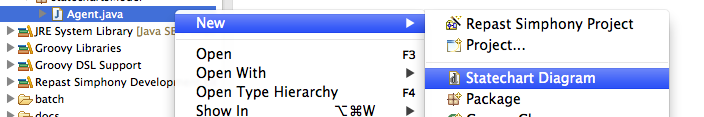
\includegraphics[width=5in]{StatechartsImages/NewStatechart.png}
}
\caption{Creating a new statechart.}
\label{fig:newStatechart}
\end{center}
\end{figure}

\begin{figure}
\begin{center}
\vspace{.2in}
\centerline {
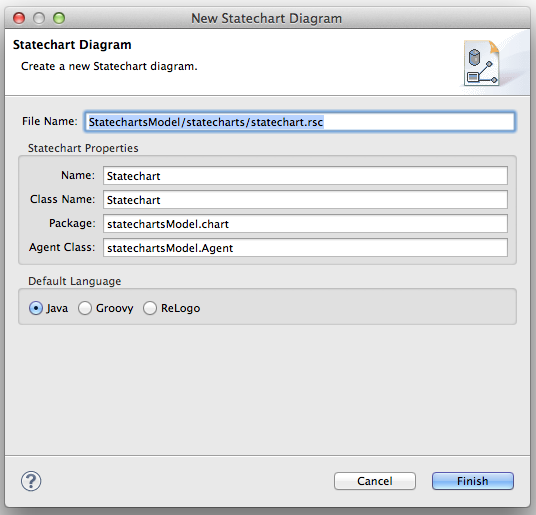
\includegraphics[width=5in]{StatechartsImages/NewStatechartWizard.png}
}
\caption{New statechart wizard.}
\label{fig:newStatechartWizard}
\end{center}
\end{figure}

After accepting or modifying the defaults, click the \emph{Finish} button. This injects a new statechart field into the selected agent class (see Listing~\ref{lst:injectedStatechart}). The \texttt{@ProbedProperty} annotation (Line~8 in Listing~\ref{lst:injectedStatechart}) connects the \emph{Name} element of the statechart to the display name that will be shown in the probe panel in the simulation runtime GUI (Section~\ref{sec:runtime}). Line~9 in Listing~\ref{lst:injectedStatechart} calls the \texttt{Statechart.createStateChart(Agent,double)} method with \texttt{0} as the second argument. This will schedule an \texttt{Agent} class's statechart to begin as soon as the \texttt{Agent} instance  is created. Alternatively, you can specify a numerical value greater than 0 (in units of simulation \emph{ticks}) to delay the statechart activation for that number of ticks. If there is a need for a statechart to begin not at a predetermined time but, for example, based on some model logic, Line~9 would be modified to read:
\begin{verbatim}Statechart statechart = Statechart.createStateChart(this);\end{verbatim}
which just instantiates the statechart but doesn't schedule it to begin at any time. Then, when the conditions for the statechart to begin are met, the statechart can be scheduled to begin with:
\begin{verbatim}StateChartScheduler.beginNow(statechart);\end{verbatim}
for immediate scheduling or:
\begin{verbatim}StateChartScheduler.beginLater(later, statechart);\end{verbatim}
for delayed scheduling at a time \texttt{later}\footnote{The statechart field does not have to be instantiated upon agent class creation. So if there is a  situation when not all of a simulation's agents will be needing their statecharts and there is a desire for conserving the simulation's memory footprint, the statechart instantiation (i.e., \texttt{Statechart.createStateChart}) can be delayed until needed.}.

\noindent\begin{minipage}[h]{\textwidth}
\vspace{.2in}
\lstset{language=java,caption=Agent class with the default injected statechart field.,label=lst:injectedStatechart}
\begin{lstlisting}
package statechartsModel;

import statechartsModel.chart.Statechart;
import repast.simphony.ui.probe.ProbedProperty;

public class Agent {

	@ProbedProperty(displayName="Statechart")
	Statechart statechart = Statechart.createStateChart(this, 0);

}
\end{lstlisting}
\vspace{.2in}
\end{minipage}

Creating a new statechart will also bring up the newly created blank statechart editor, which we describe next.





\clearpage

\subsection{Statecharts Editor}

The statecharts editor is divided into three main panels (Figure~\ref{fig:statechartEditorBoxes}). The first (Figure~\ref{fig:statechartEditorBoxes}a) is the statecharts workspace area. This is where the visual elements of a statechart are created and arranged. The palette panel (Figure~\ref{fig:statechartEditorBoxes}b) shows the available statechart elements that can be used in the statecharts workspace\footnote{Sections~\ref{sec:states} and \ref{sec:transitions} will cover these elements in detail.} Clicking on an element in the palette panel and then clicking on the statecharts workspace will create an instance of that element in the workspace. The properties panel (Figure~\ref{fig:statechartEditorBoxes}c) shows the properties of the element selected in the statecharts workspace. If, as in Figure~\ref{fig:statechartEditorBoxes}, no element is selected, the properties of the statechart itself are shown. In addition to displaying element properties, the panel is also where the properties of elements can be edited. A statechart has a priority which indicates the order in which it will be resolved with respect to other statecharts (see red box in Figure~\ref{fig:statechartProperties}). So, for example, if an agent has two statecharts (A and B) and statechart A should be resolved before statechart B, giving statechart A a higher priority will ensure that this occurs.
\begin{figure}
\begin{center}
\vspace{.2in}
\centerline {
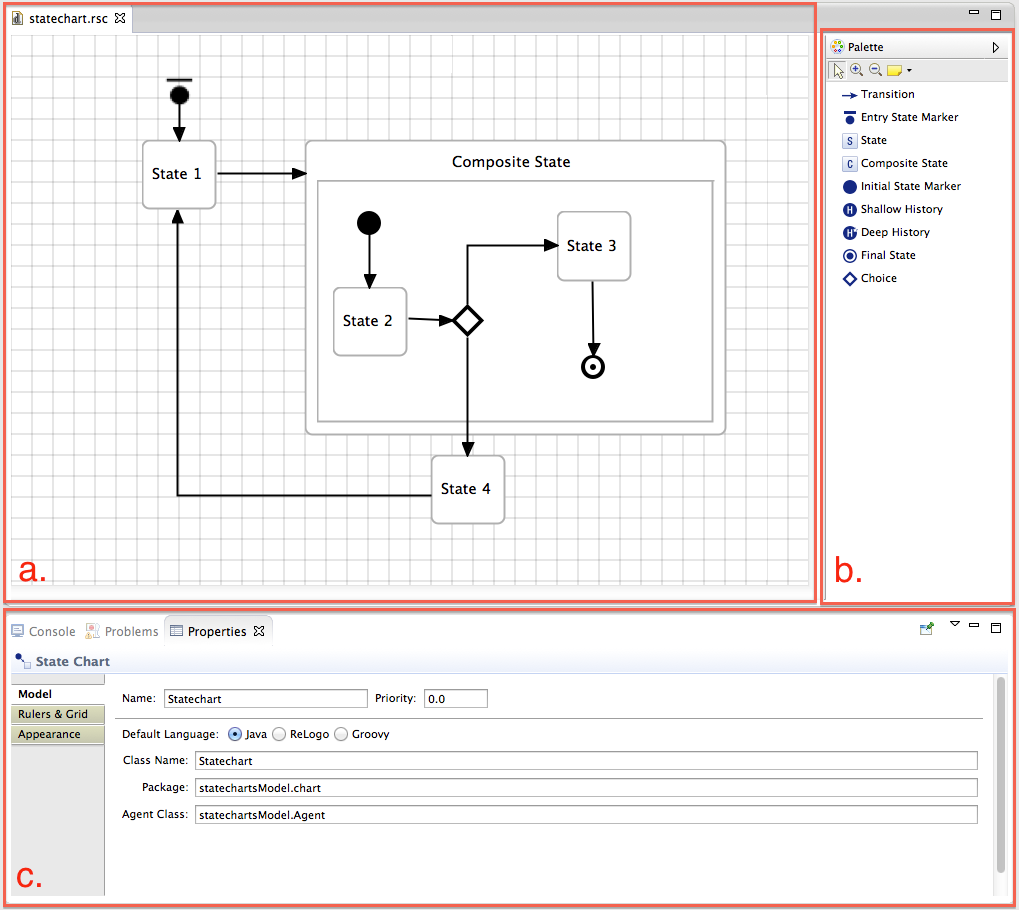
\includegraphics[width=5in]{StatechartsImages/StatechartEditorBoxes.png}
}
\caption{The components of the statecharts visual editor. a)~The workspace area where the statechart elements are created and arranged. b)~The palette panel of available elements, including selection, zoom and note tools. c)~The properties panel of the selected statechart element in the workspace (a). If no element is selected, the properties of the statechart itself are displayed.}
\label{fig:statechartEditorBoxes}
\end{center}
\end{figure}

\begin{figure}
\begin{center}
\vspace{.2in}
\centerline {
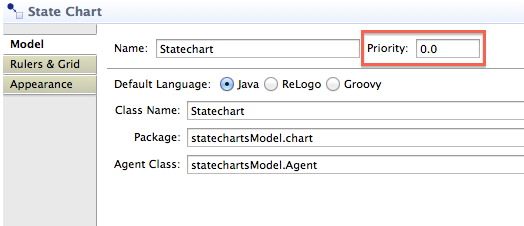
\includegraphics[width=5in]{StatechartsImages/StatechartProperties.png}
}
\caption{The statechart properties panel with the priority element indicated by a red box.}
\label{fig:statechartProperties}
\end{center}
\end{figure}

There is a contextual menu approach for adding elements to the workspace as well. Simply hovering over an area in the workspace will reveal a contextual menu of the available elements appropriate for the region pointed to. If the mouse pointer is on an empty space in the workspace background, you will see the contextual menu in Figure~\ref{fig:defaultContextualMenu}. If the pointer is on a state, you will see transitions shortcuts like in Figure~\ref{fig:stateConnectorsHover}, the left symbol indicating a connection from this state and the right symbol a connection to this state. Finally, if the pointer is inside a composite state, you will see the contextual menu in Figure~\ref{fig:compositeContextualMenu}.


\begin{figure}

\begin{center}
\vspace{.2in}
\centerline {
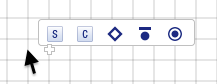
\includegraphics[height=1in]{StatechartsImages/DefaultContextualMenu.png}
}
\caption{The default contextual menu when the pointer is on a blank area of the workspace.}
\label{fig:defaultContextualMenu}
\end{center}
\end{figure}

\begin{figure}
\begin{center}
\vspace{.2in}
\centerline {
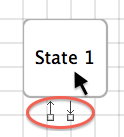
\includegraphics[height=1in]{StatechartsImages/StateConnectorsHover.png}
}
\caption{The transitions shortcuts, circled in red, for making connections from (left) and to (right) the state.}
\label{fig:stateConnectorsHover}
\end{center}
\end{figure}
\begin{figure}
\begin{center}
\vspace{.2in}
\centerline {
\includegraphics[height=2in]{StatechartsImages/CompositeContextualMenu.png}
}
\caption{The contextual menu when the pointer is inside a composite state.}
\label{fig:compositeContextualMenu}
\end{center}

\end{figure}

\clearpage

\section{States}
\label{sec:states}
One of the fundamental building blocks of statecharts are states. Here we introduce the different types of states that exist within the Repast Simphony statecharts framework.

\subsection{Entry State Marker}

\includegraphics[height=.2in]{StatechartsImages/First-State-32.png}

Every statechart must have an entry state marker. This defines point of entry into a statechart takes when the statechart is activated.

\subsection{Simple State}
\label{sec:simpleState}

\includegraphics[height=.2in]{StatechartsImages/State-32.png}

A simple state looks like Figure~\ref{fig:simpleState}. At any one point in time within an active statechart, one and only one of the simple states will be active. In addition to their \emph{ID}, simple states can have \emph{On Enter} and \emph{On Exit} actions defined, as seen in the simple state properties panel in Figure~\ref{fig:simpleStateProperties}. These actions are triggered when entering or exiting the simple state, respectively. The keywords available within the two action blocks are:
\begin{description}
\item[agent] This is the agent that contains the statechart. Any method (e.g., \texttt{customMethod}) defined on the agent can be invoked through this reference (e.g., \texttt{agent.customMethod()}).
\item[state] This is the state itself. For example, the state's \emph{ID} can be accessed via \texttt{state.getId()}.
\item[params] This is the model's \texttt{Parameters} object. As an example, a double valued parameter \texttt{dParam} can be retrieved with: \texttt{params.getDouble("dParam")}\footnote{See the source or JavaDoc for  \texttt{repast.simphony.parameter.Parameters} for all of the available methods.}.
\end{description}

As is the case with all types of action blocks, their logic can be specified using Java, Groovy or ReLogo. Specifically, any Java, Groovy or ReLogo code can be used to express the behavior that should be executed upon entry to or exit from the state\footnote{When using the ReLogo option, the \texttt{agent} parameter is implicit so writing \texttt{customMethod()} is equivalent to \texttt{agent.customMethod()}.}.

\begin{figure}
\begin{center}
\vspace{.2in}
\centerline {
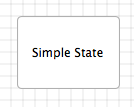
\includegraphics[width=1in]{StatechartsImages/SimpleState.png}
}
\caption{Simple state.}
\label{fig:simpleState}
\end{center}
\end{figure}

\begin{figure}
\begin{center}
\vspace{.2in}
\centerline {
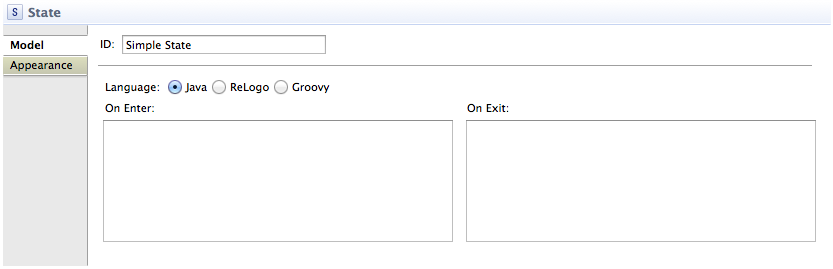
\includegraphics[width=5in]{StatechartsImages/SimpleStateProperties.png}
}
\caption{Simple state properties.}
\label{fig:simpleStateProperties}
\end{center}
\end{figure}

\clearpage

\subsection{Composite State}
\label{sec:compositeState}

\includegraphics[height=.2in]{StatechartsImages/Composite-State-32.png}

Composite states are used to nest elements within a statechart. Figure~\ref{fig:compositeState} shows an empty composite state and Figure~\ref{fig:compositeStateProperties} shows the properties panel for composite states, which is identical to that of the simple states in that \emph{On Enter} and \emph{On Exit} actions can be defined. The difference between composite and simple states lies in the fact that composite states can include the following elements as sub-elements:
\begin{itemize}
\item Simple state (Section~\ref{sec:simpleState})
\item Composite state (Section~\ref{sec:compositeState})
\item Initial state marker (Section~\ref{sec:initialStateMarker})
\item History state (Section~\ref{sec:historyState})
\item Final state (Section~\ref{sec:finalState})
\item Branching state (Section~\ref{sec:branchingState})
\end{itemize}
Whenever a sub-element is active, the composite state containing that sub-element will be active as well. If a transition is made from outside of a composite state directly to a sub-element, the composite state will be entered prior to its sub-elements. In a similar manner, if a transition is followed from a sub-element out of the composite state, the composite state will be exited after the sub-elements are exited.

\begin{figure}
\begin{center}
\vspace{.2in}
\centerline {
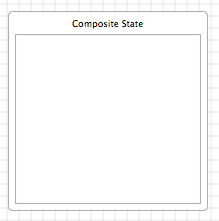
\includegraphics[width=2in]{StatechartsImages/CompositeState.png}
}
\caption{Composite state.}
\label{fig:compositeState}
\end{center}
\end{figure}

\begin{figure}
\begin{center}
\vspace{.2in}
\centerline {
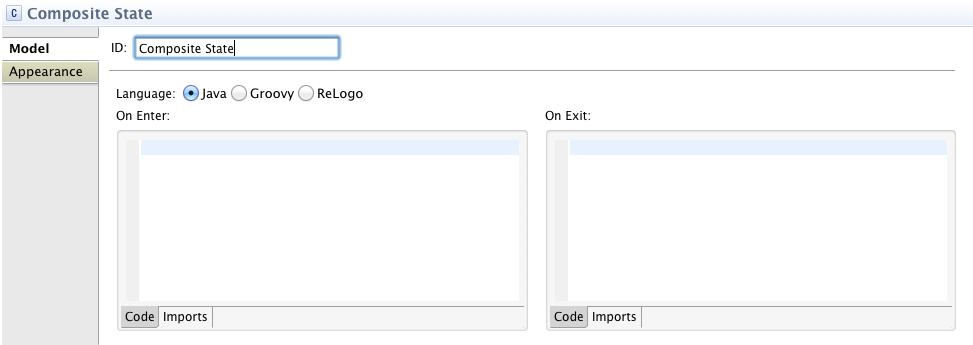
\includegraphics[width=5in]{StatechartsImages/CompositeStateProperties.png}
}
\caption{Composite state properties.}
\label{fig:compositeStateProperties}
\end{center}
\end{figure}

\clearpage

\subsection{Initial State Marker}
\label{sec:initialStateMarker}

\includegraphics[height=.2in]{StatechartsImages/Initial-State-32.png}

Any composite state that has a transition ending at it or contains history states must define an initial state marker. The initial state marker points to the element within the composite state that should be entered upon entering the composite state.

\begin{figure}
\begin{center}
\vspace{.2in}
\centerline {
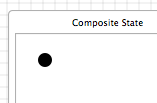
\includegraphics[width=1.5in]{StatechartsImages/InitialStateMarker.png}
}
\caption{Initial state marker (within a composite state).}
\label{fig:initialStateMarker}
\end{center}
\end{figure}


\subsection{History State}
\label{sec:historyState}

\includegraphics[height=.2in]{StatechartsImages/Shallow-History-32.png} 
\includegraphics[height=.2in]{StatechartsImages/Deep-History-32.png}

There are two types of history states, shallow and deep (Figure~\ref{fig:history}). When a shallow history state is entered, the last active element within the enclosing composite state at the same hierarchical level of the history state is re-entered. For a deep history state, the last active \emph{simple state} within the enclosing composite state, no matter at what level of the nesting hierarchy, is entered. In both cases if there was no previously active state, the state pointed to by the initial state marker is entered. Figure~\ref{fig:historyProperties} shows the properties panel for a (shallow) history state. Only an \emph{On Enter} element can be defined since history states are never directly exited.


\begin{figure}
\begin{center}
\vspace{.2in}
\centerline {
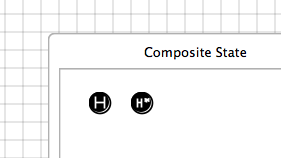
\includegraphics[width=2in]{StatechartsImages/History.png}
}
\caption{Shallow (left) and deep (right) history states (within a composite state).}
\label{fig:history}
\end{center}
\end{figure}

\begin{figure}
\begin{center}
\vspace{.2in}
\centerline {
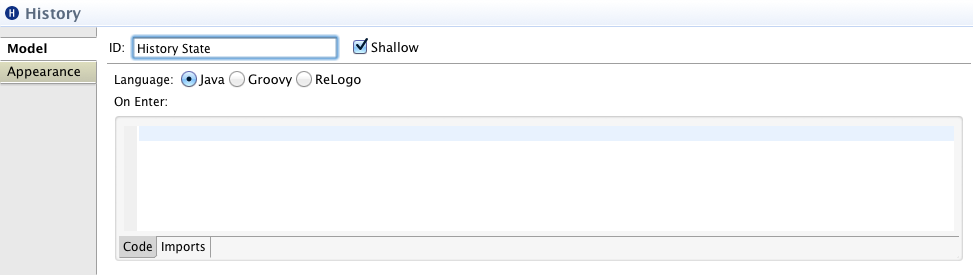
\includegraphics[width=5in]{StatechartsImages/HistoryProperties.png}
}
\caption{The properties panel for a shallow history state. A deep history state would have the same properties panel except that the \emph{Shallow} element would be unchecked.}
\label{fig:historyProperties}
\end{center}
\end{figure}

\clearpage

\subsection{Final State}
\label{sec:finalState}

\includegraphics[height=.2in]{StatechartsImages/Final-State-32.png}
A final state marks the end of all activities for a statechart. When a final state is entered, no further states will be visited and no transitions will be triggered. Figure~\ref{fig:finalProperties} shows the properties panel for a final state. Only an \emph{On Enter} element can be defined since final states are never exited.

\begin{figure}
\begin{center}
\vspace{.2in}
\centerline {
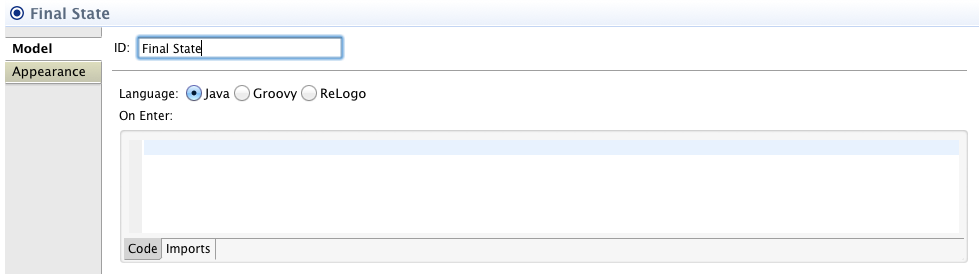
\includegraphics[width=5in]{StatechartsImages/FinalProperties.png}
}
\caption{The properties panel for a final state.}
\label{fig:finalProperties}
\end{center}
\end{figure}

\clearpage

\subsection{Branching State}
\label{sec:branchingState}

\includegraphics[height=.2in]{StatechartsImages/Choice-32.png}

Branching states represent logical branching within statecharts (Figure~\ref{fig:branching}). Every branching state must define one outgoing \emph{Default} transtion, where the rest of the outgoing transitions are \emph{Condition} transitions (Section~\ref{sec:conditionTransition}). The \emph{Condition} transitions are checked for validity and, if valid conditions are found, the transitions' priorities dictate the transition that is followed. If no valid transitions are found, the \emph{Default} transition is followed. Figure~\ref{fig:branchingProperties} shows the properties panel for a branching state. Since a branching state is entered and immediately exited, nothing other than the state's \emph{ID} can be specified.

\begin{figure}
\begin{center}
\vspace{.2in}
\centerline {
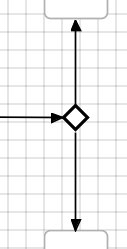
\includegraphics[width=1in]{StatechartsImages/Branching.png}
}
\caption{A branching state with one incoming and two outgoing transitions.}
\label{fig:branching}
\end{center}
\end{figure}

\begin{figure}
\begin{center}
\vspace{.2in}
\centerline {
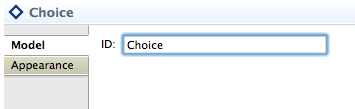
\includegraphics[width=3in]{StatechartsImages/BranchingProperties.png}
}
\caption{The properties panel for a branching state.}
\label{fig:branchingProperties}
\end{center}
\end{figure}

\clearpage

\section{Transitions}
\label{sec:transitions}

Transitions between states make up the other fundamental building block of statecharts. In this section we introduce the different types of transitions that can be used within the Repast Simphony statecharts framework.

There are two overall types of transitions, \emph{regular transitions} (Figure~\ref{fig:regularTransition}) which connect different states and \emph{self transitions} (Figure~\ref{fig:selfTransition}) which are internal to a state\footnote{One also has the ability to define a \emph{regular transition} that begins and ends at the same state. Unlike the \emph{self transition} case, each time the \emph{regular transition} is taken, the state will be exited and subsequently re-entered.}. There are a number of different transition trigger types, demonstrated in the transition properties panel in Figure~\ref{fig:transitionProperties} (these will be discussed below in further detail).

For any transition an \emph{On Transition} action can be defined (see Figure~\ref{fig:transitionPropertiesOnTransition}). This action will be executed whenever the transition is traversed. The keywords available within the \emph{On Transition} action block are:
\begin{description}
\item[agent] This is the agent that contains the statechart.
\item[transition] This is the transition itself. For example, the transition's source state can be accessed via: \texttt{transition.getSource()}\footnote{See the source or JavaDoc for \texttt{repast.simphony.statecharts.Transition} for all of the available methods.}.
\item[params] This is the model's \texttt{Parameters} object.
\end{description}

\begin{figure}
\begin{center}
\vspace{.2in}
\centerline {
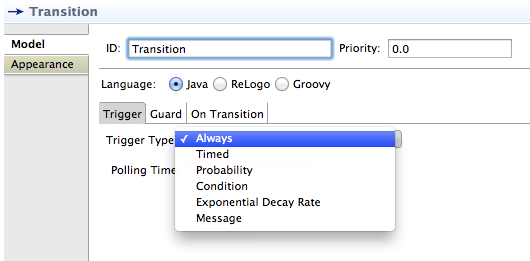
\includegraphics[width=4in]{StatechartsImages/TransitionProperties.png}
}
\caption{The properties panel showing the different types of transitions that are available.}
\label{fig:transitionProperties}
\end{center}
\end{figure}


For almost all types of transitions\footnote{All transitions except default transitions out of branching states.} a \emph{Guard} condition can be defined (see Figure~\ref{fig:transitionPropertiesGuard}). A \emph{Guard} condition is an additional boolean condition that has to be satisfied for a transition that is valid to be actually considered as a candidate for traversal. This condition is specified by a block of code that returns a boolean and the keywords available in a \emph{Guard} condition are the same as those in an \emph{On Transition} action block.

When there is more than one valid transition ties are broken using the priority of the transition. If the priorities of valid transitions are equal then one of the transitions will be chosen with a uniform random probability. The priority of a transition can be specified in the transition's properties panel.

\emph{Regular transitions} can be divided into zero time transitions and non-zero time transitions\footnote{All \emph{self transitions} are non-zero time transitions.}. For zero time transitions when a new state is entered, if there is a valid zero time transition out of it, that transition is followed immediately (with ties broken via priorities as usual). Always (Section~\ref{sec:alwaysTransition}), Condition (Section~\ref{sec:conditionTransition}) and Message (Section~\ref{sec:messageTransition}) transition triggers are zero-time transitions.

Within a state, transitions are resolved starting with \emph{self transitions} and proceeded by \emph{regular transitions}.

Every transition has a \emph{polling time} associated with it. This indicates the frequency (in units of simulation \emph{ticks}) with which the transition is polled for validity.

Next we present the different transition trigger types in more detail.

\begin{figure}

\begin{minipage}{.5\textwidth}
\begin{center}
\vspace{.2in}
\centerline {
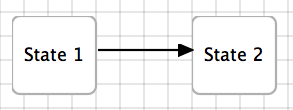
\includegraphics[height=1in]{StatechartsImages/RegularTransition.png}
}
\caption{Regular transition between states 1 and 2.}
\label{fig:regularTransition}
\end{center}
\end{minipage}%
\begin{minipage}{.5\textwidth}
\begin{center}
\vspace{.2in}
\centerline {
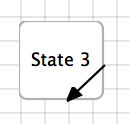
\includegraphics[height=1in]{StatechartsImages/SelfTransition.png}
}
\caption{Self transition internal to State 3.}
\label{fig:selfTransition}
\end{center}
\end{minipage}

\end{figure}

\begin{figure}
\begin{center}
\vspace{.2in}
\centerline {
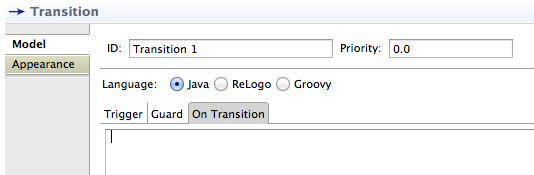
\includegraphics[height=1.6in]{StatechartsImages/TransitionPropertiesOnTransition.png}
}
\caption{Properties panel for a transition showing the \emph{On Transition} action block.}
\label{fig:transitionPropertiesOnTransition}
\end{center}
\end{figure}

\begin{figure}
\begin{center}
\vspace{.2in}
\centerline {
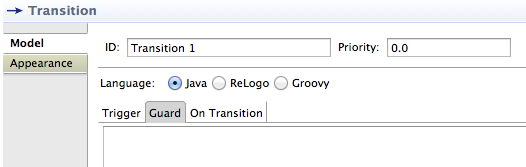
\includegraphics[height=1.6in]{StatechartsImages/TransitionPropertiesGuard.png}
}
\caption{Properties panel for a transition showing the \emph{Guard} condition block.}
\label{fig:transitionPropertiesGuard}
\end{center}

\end{figure}


%\begin{figure}
%
%\begin{minipage}{.5\textwidth}
%\begin{center}
%\vspace{.2in}
%\centerline {
%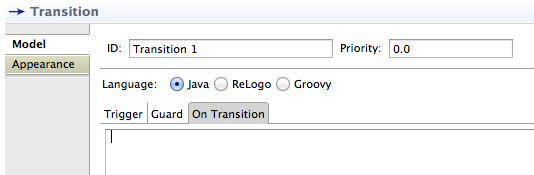
\includegraphics[height=0.8in]{StatechartsImages/TransitionPropertiesOnTransition.png}
%}
%\caption{Properties panel for a transition showing the \emph{On Transition} action block.}
%\label{fig:transitionPropertiesOnTransition}
%\end{center}
%\end{minipage}%
%\begin{minipage}{.5\textwidth}
%\begin{center}
%\vspace{.2in}
%\centerline {
%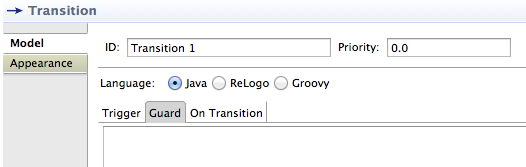
\includegraphics[height=0.8in]{StatechartsImages/TransitionPropertiesGuard.png}
%}
%\caption{Properties panel for a transition showing the \emph{Guard} condition block.}
%\label{fig:transitionPropertiesGuard}
%\end{center}
%\end{minipage}
%
%\end{figure}
\clearpage

\subsection{Always Trigger}
\label{sec:alwaysTransition}
\emph{Always} triggers are always valid. The transition can, however, contain a \emph{Guard} condition which if false, would prevent the transition from triggering. Because this trigger type results in zero time transitions, it is important to make sure that there are no \emph{always} trigger transitions contributing to zero time loops in any statechart you create, since this has the potential to create never-ending loops. The properties panel for an \emph{always} trigger transition is in Figure~\ref{fig:alwaysTransitionProperties}. One use for \emph{always} trigger transitions is as self transitions to execute some action at a set polling time.

\begin{figure}
\begin{center}
\vspace{.2in}
\centerline {
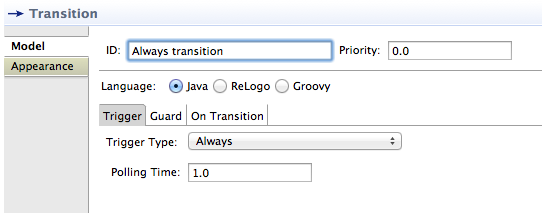
\includegraphics[width=4in]{StatechartsImages/AlwaysTransitionProperties.png}
}
\caption{The properties panel for an \emph{always} transition.}
\label{fig:alwaysTransitionProperties}
\end{center}
\end{figure}
\clearpage

\subsection{Timed Trigger}
\label{sec:timedTransition}
\emph{Timed} triggers become valid after some time, measured in simulation \emph{ticks}. The properties panel for a \emph{timed} trigger transition is shown in Figure~\ref{fig:timedTransitionProperties}. The \emph{Time} element in the properties panel accepts general Java, Groovy or ReLogo code returning a numerical value, including simple numerical entries (e.g., \texttt{2} or \texttt{agent.getDelay()}), with the same keywords as the \emph{On Transition} action block (i.e., \texttt{agent}, \texttt{transition}, \texttt{params}). If at the time a \emph{timed} trigger is valid a \emph{Guard} condition keeps the transition from being valid, the transition does not get reinitialized and will simply remain invalid.

\begin{figure}
\begin{center}
\vspace{.2in}
\centerline {
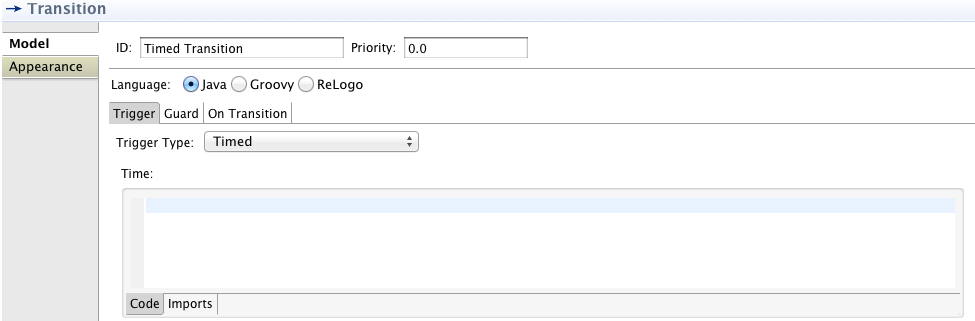
\includegraphics[width=5in]{StatechartsImages/TimedTransitionProperties.png}
}
\caption{The properties panel for a \emph{timed} transition.}
\label{fig:timedTransitionProperties}
\end{center}
\end{figure}
\clearpage


\subsection{Probability Trigger}
\emph{Probability} triggers are evaluated as valid with a specified probability. The properties panel for a \emph{probability} trigger transition is shown in Figure~\ref{fig:probabilityTransitionProperties}. The \emph{Probability} element in the properties panel accepts general Java, Groovy or ReLogo code returning a numerical value, including simple numerical entries (e.g., \texttt{0.2} or \texttt{agent.getProbability()}), with the same keywords as the \emph{On Transition} action block (i.e., \texttt{agent}, \texttt{transition}, \texttt{params}). The code block is evaluated each time the transition is polled for validity.

\begin{figure}
\begin{center}
\vspace{.2in}
\centerline {
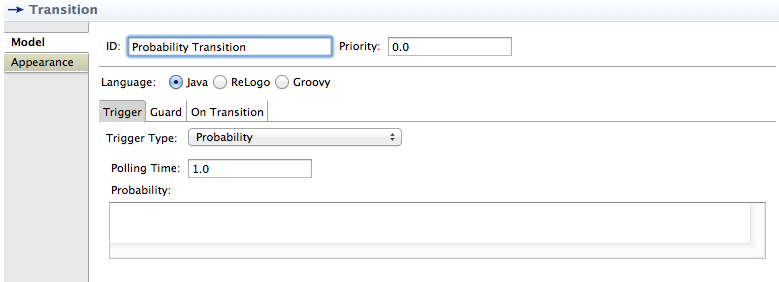
\includegraphics[width=5in]{StatechartsImages/ProbabilityTransitionProperties.png}
}
\caption{The properties panel for a \emph{probability} transition.}
\label{fig:probabilityTransitionProperties}
\end{center}
\end{figure}
\clearpage

\subsection{Condition Trigger}
\label{sec:conditionTransition}
\emph{Condition} triggers are evaluated as valid based on a specified condition. The properties panel for a \emph{condition} trigger transition is shown in Figure~\ref{fig:conditionTransitionProperties}. The \emph{Condition} element in the properties panel accepts general Java, Groovy or ReLogo code returning a boolean value, including simple boolean entries (e.g., \texttt{true} or \texttt{agent.getCondition()}), with the same keywords as the \emph{On Transition} action block (i.e., \texttt{agent}, \texttt{transition}, \texttt{params}). The code block is evaluated each time the transition is polled for validity.

\begin{figure}
\begin{center}
\vspace{.2in}
\centerline {
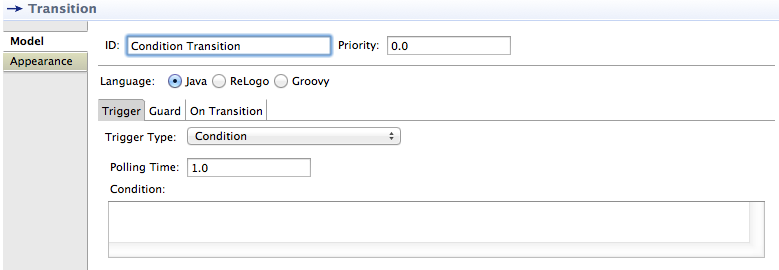
\includegraphics[width=5in]{StatechartsImages/ConditionTransitionProperties.png}
}
\caption{The properties panel for a \emph{condition} transition.}
\label{fig:conditionTransitionProperties}
\end{center}
\end{figure}
\clearpage


\subsection{Exponential Decay Rate Trigger}
\emph{Exponential decay rate} triggers become valid after a random time following the exponential distribution. The properties panel for an \emph{exponential decay rate} trigger transition is shown in Figure~\ref{fig:exponentialTransitionProperties}. The \emph{Exponential Decay Rate} element in the properties panel accepts general Java, Groovy or ReLogo code returning a numerical value, including simple numerical entries (e.g., \texttt{2} or \texttt{agent.getDecayRate()}), with the same keywords as the \emph{On Transition} action block (i.e., \texttt{agent}, \texttt{transition}, \texttt{params}). The code block is evaluated when the transition is initialized (i.e., when a state is entered that has a possible \emph{exponential decay rate} transition leading out of it). The code block supplies the $\lambda$ parameter to the exponential distribution specified by the probability density function:
\begin{equation}
f(t) = \lambda e^{-\lambda t}
\end{equation}
The expected value of an exponentially distributed random variable with parameter $\lambda$ is $1/\lambda$. So given, for example, a $\lambda$ of 2, the expected value for the time it would take for an \emph{exponential decay rate} transition to trigger would be 0.5 in units of simulation \emph{ticks}.

\begin{figure}
\begin{center}
\vspace{.2in}
\centerline {
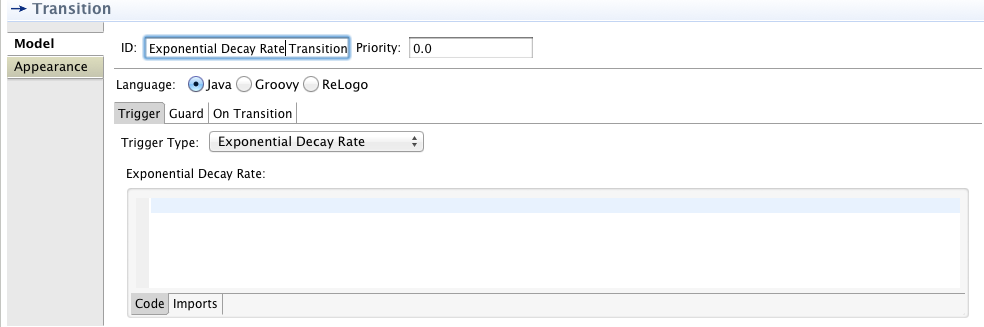
\includegraphics[width=5in]{StatechartsImages/ExponentialTransitionProperties.png}
}
\caption{The properties panel for a \emph{exponential decay rate} transition.}
\label{fig:exponentialTransitionProperties}
\end{center}
\end{figure}
\clearpage



\subsection{Message Trigger}
\label{sec:messageTransition}
\emph{Message} triggers become valid when a message meeting specific criteria is received by the statechart. A statechart is sent a message when the statechart's \texttt{receiveMessage(Object)} method is called. From an agent-based modeling perspective, this would likely occur when an agent is sent a message and then the agent forwards the message to all or a subset of its statecharts\footnote{There is nothing to prevent one agent from directly accessing another agent's statechart if the statechart is visible, but it could be considered not very good practice in an object oriented programming sense.}. Messages from the queue are consumed by message transitions in the order they were received. If there are message transitions to check, the queue will be checked until a valid message is found.

There are four different types of \emph{message} triggers, shown in the drop down menu of the \emph{Trigger} element in the \emph{message} trigger properties pane in Figure~\ref{fig:messageTransitionProperties}, and we present them next.

\begin{figure}
\begin{center}
\vspace{.2in}
\centerline {
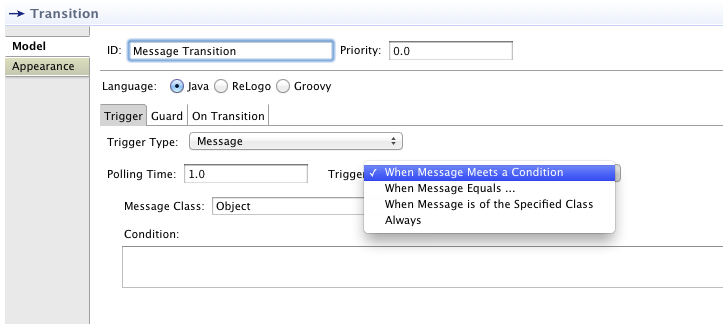
\includegraphics[width=5in]{StatechartsImages/MessageTransitionProperties.png}
}
\caption{The properties panel for a \emph{message} message, with the available trigger types shown under the \emph{Trigger} element.}
\label{fig:messageTransitionProperties}
\end{center}
\end{figure}
\clearpage

\subsubsection{When Message Meets Condition}
The \emph{When Message Meets a Condition} message trigger has the properties panel shown in Figure~\ref{fig:message1TransitionProperties}. The \emph{Message Class} element is specifies the type of the message, which can be any of the basic types in Figure~\ref{fig:messageClassType} or the fully qualified name of any another type\footnote{The default \emph{Message Class} is \texttt{java.lang.Object} which will accept any type of message.}. To specify a type not in the list, enter the fully qualified name of the type in the combo box. The \emph{Condition} element in the properties panel accepts general Java, Groovy or ReLogo code returning a boolean value, including simple boolean entries (e.g., \texttt{true} or \texttt{agent.getCondition()}). The keywords available within the \emph{Condition} action block are:
\begin{description}
\item[agent] This is the agent that contains the statechart.
\item[transition] This is the transition itself.
\item[message] This is the message received by the statechart.
\item[params] This is the model's \texttt{Parameters} object.
\end{description}
The code block is evaluated each time the transition is polled for validity.

\begin{figure}
\begin{center}
\vspace{.2in}
\centerline {
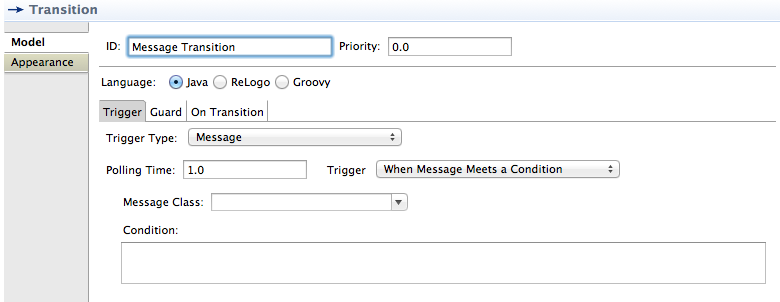
\includegraphics[width=5in]{StatechartsImages/Message1TransitionProperties.png}
}
\caption{The properties panel for a \emph{When Message Meets a Condition} message trigger.}
\label{fig:message1TransitionProperties}
\end{center}
\end{figure}

\begin{figure}
\begin{center}
\vspace{.2in}
\centerline {
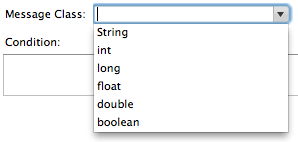
\includegraphics[width=3.0in]{StatechartsImages/MessageClassType.png}
}
\caption{The basic types available for the \emph{Message Class} element in the properties panel for the \emph{When Message Meets a Condition}, \emph{When Message Equals}, and \emph{When Message is of the Specified Class} message triggers. Additional types can be specified with their fully qualified names.}
\label{fig:messageClassType}
\end{center}
\end{figure}
\clearpage


\subsubsection{When Message Equals}
The \emph{When Message Equals} message trigger has the properties panel shown in Figure~\ref{fig:message2TransitionProperties}. The only difference between this and the \emph{When Message Meets a Condition} message trigger is that instead of a \emph{Condition} element there is an \emph{Equals} element that needs to be defined. The \emph{Equals} element accepts general Java, Groovy or ReLogo code returning any value that will be checked against the received message using the message's \texttt{equals(Object)} method. The keywords within the \emph{Equals} block are the same as the \emph{On Transition} action block (i.e., \texttt{agent}, \texttt{transition}, \texttt{params}).

\begin{figure}
\begin{center}
\vspace{.2in}
\centerline {
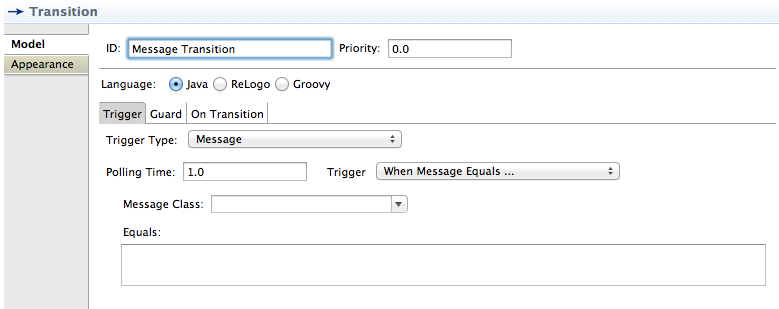
\includegraphics[width=5in]{StatechartsImages/Message2TransitionProperties.png}
}
\caption{The properties panel for a \emph{When Message Equals} message trigger.}
\label{fig:message2TransitionProperties}
\end{center}
\end{figure}
\clearpage


\subsubsection{When Message is of Class}
The \emph{When Message is of Class} message trigger has the properties panel shown in Figure~\ref{fig:message3TransitionProperties}. Any message that is received that is of the specified class type will result in the transition being triggered.

\begin{figure}
\begin{center}
\vspace{.2in}
\centerline {
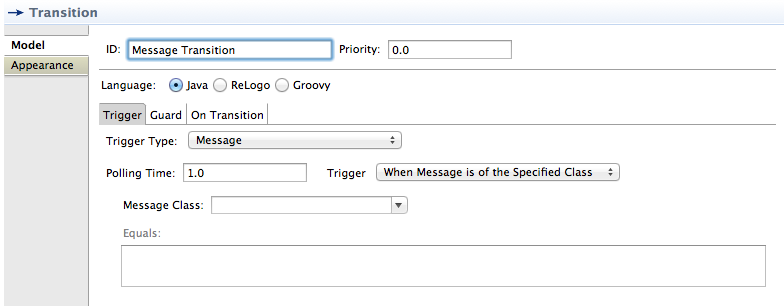
\includegraphics[width=5in]{StatechartsImages/Message3TransitionProperties.png}
}
\caption{The properties panel for a \emph{When Message is of Class} message trigger.}
\label{fig:message3TransitionProperties}
\end{center}
\end{figure}

\subsubsection{Always}

The \emph{Always} message trigger has the properties panel shown in Figure~\ref{fig:message4TransitionProperties}. Any message that is received will result in the transition being triggered.

\begin{figure}
\begin{center}
\vspace{.2in}
\centerline {
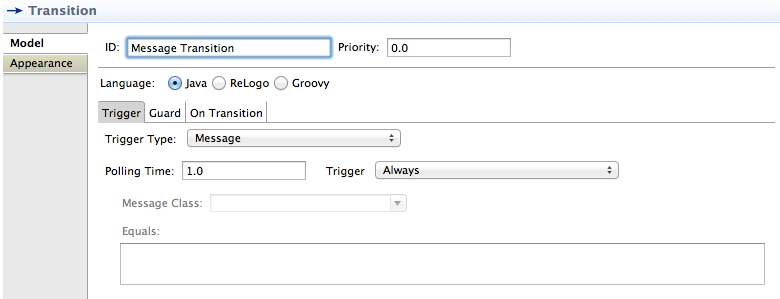
\includegraphics[width=5in]{StatechartsImages/Message4TransitionProperties.png}
}
\caption{The properties panel for an \emph{Always} message trigger.}
\label{fig:message4TransitionProperties}
\end{center}
\end{figure}
\clearpage

\section{Debugging Statecharts}
When a statechart is saved the code for that statechart will be generated in the \texttt{src-gen} directory in the statechart's project. At that time the statechart will also be validated and any structural warnings or errors will be displayed in the statechart workspace.  Figure \ref{fig:transitionerror} is an example of this. The transition between State 0 and State 2 has an error. Moving the mouse pointer over the error marker will display a tooltip with the error message. In this case, the transition has a \emph{Condition} trigger type but no condition has been specified in the transition's properties. The error message will also be displayed in Eclipse's \emph{Problems} view. 

\begin{figure}
\begin{center}
\vspace{.2in}
\centerline {
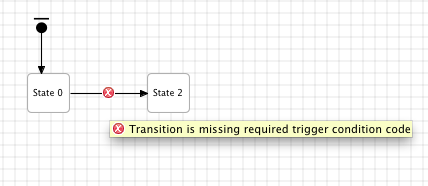
\includegraphics[width=5in]{StatechartsImages/transition_error.png}
}
\caption{An error marker on a transition}
\label{fig:transitionerror}
\end{center}
\end{figure}


If there is an error in the code generated by the statechart, you will see the error marker on the src-gen folder in the statechart's project. This kind of error will occur when any code specified in the statechart's state or transition properties (such as the \emph{On Exit}, \emph{Condition} and so forth code blocks) is erroneous. To fix these kind of errors, expand the src-gen folder to find the offending file as in Figure~\ref{fig:srcgen}. Open the file. The comments in the file describe the statechart element that produced the bad code and eclipse will flag errors in the code itself. Figure \ref{fig:codeerror} shows such an error. The error itself is that the \texttt{getHealt} method is not defined on the agent. The comments in the code state that this is the code for the ``Condition trigger condition for Transition 3, from = State 0, to = State 2.'' To fix this then, we need to edit the trigger condition code in Transition 3.  To find it, we  can use the \emph{to} and \emph{from} states mentioned in the comments and select the transition that connects them.  Note that editing the code directly in the .java file will remove the error, but will \textbf{NOT} fix the problem. The next time the statechart is saved, the code will be regenerated. The code must be fixed in the statechart element that produced the problem.


\begin{figure}
\begin{center}
\vspace{.2in}
\centerline {
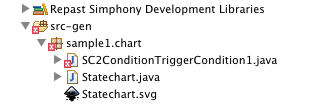
\includegraphics[width=5in]{StatechartsImages/srcgen_error.png}
}
\caption{An example of an error in the code generated from the statechart.}
\label{fig:srcgen}
\end{center}
\end{figure}

\begin{figure}
\begin{center}
\vspace{.2in}
\centerline {
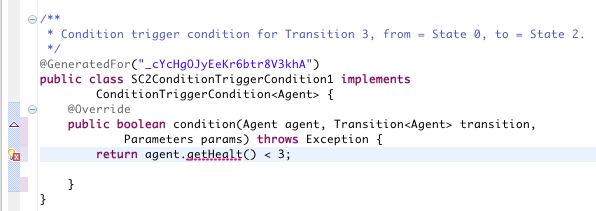
\includegraphics[width=5.5in]{StatechartsImages/code_error.png}
}
\caption{An error in the code produced by the statechart. Note that the comments refer to the element that produced the code.}
\label{fig:codeerror}
\end{center}
\end{figure}


\section{Statecharts at Runtime}
\label{sec:runtime}
When a simulation is running, an agent's statechart can be visually accessed via the agent's probe panel. An agent's probe panel is launched by double clicking an agent in a display within the Repast Simphony runtime GUI. Figure~\ref{fig:probe} shows the Repast Simphony runtime GUI with a gridded display on the right and a probe panel on the bottom left (larger red rectangle). The probe panel was launched by double-clicking the visible agent on the right (blue filled circle). Within the probe panel, the button to display the \emph{Statechart} statechart is indicated with the smaller red rectangle (and the red arrow). When this button is pressed, a statechart display is launched (Figure~\ref{fig:runtimeStatechart}). The statechart display highlights active states with a green color\footnote{As seen in Figure~\ref{fig:runtimeStatechart}, a composite state is active if a sub-element is active (unless the sub-element is a final state).}. Under the statechart display \emph{Options} menu item there is a menu item (\emph{Always On Top}) to always keep the statecharts display on top of other displays. This is enabled by default but can be disabled.

\begin{figure}
\begin{center}
\vspace{.2in}
\centerline {
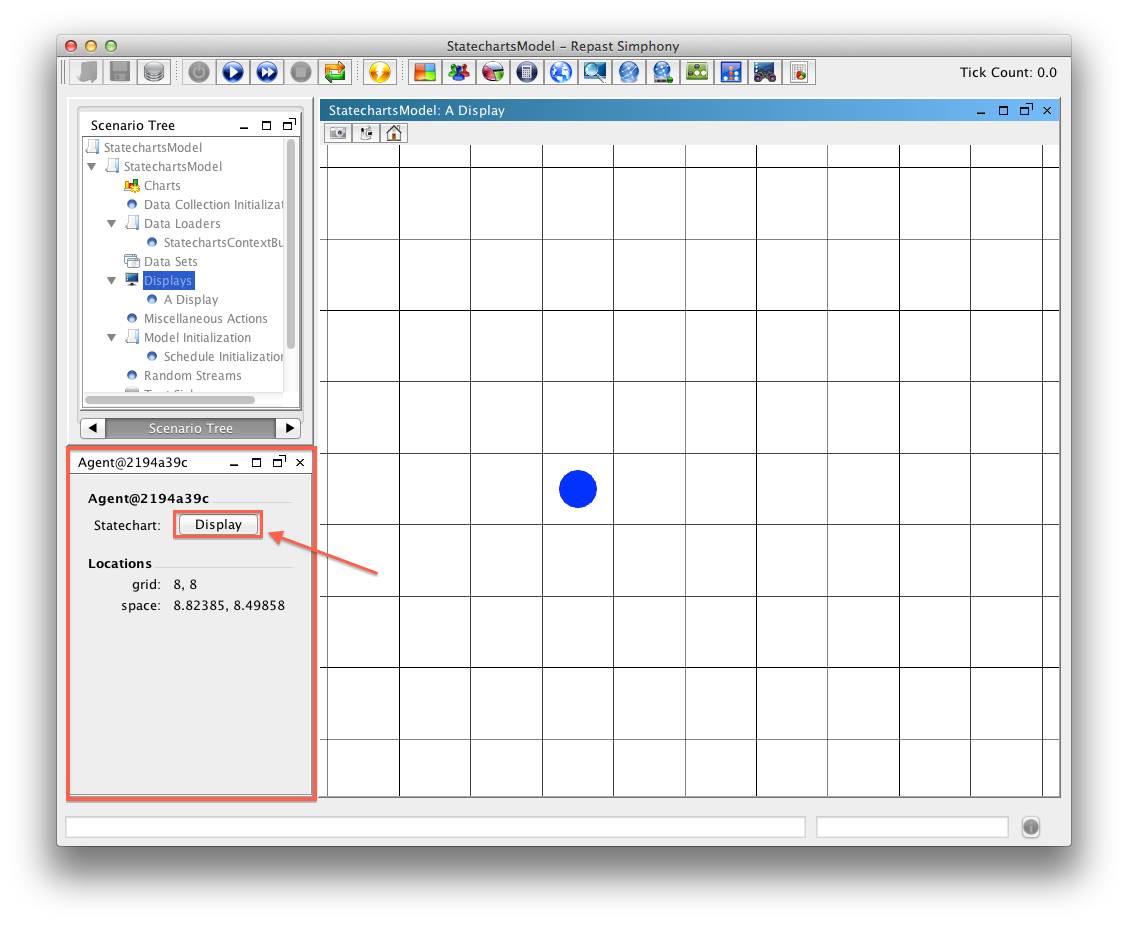
\includegraphics[width=5in]{StatechartsImages/Probe.png}
}
\caption{Repast Simphony runtime GUI with a probe panel showing (large red rectangle) and with a statechart display button (smaller red rectangle with arrow pointing to it).}
\label{fig:probe}
\end{center}
\end{figure}

\begin{figure}
\begin{center}
\vspace{.2in}
\centerline {
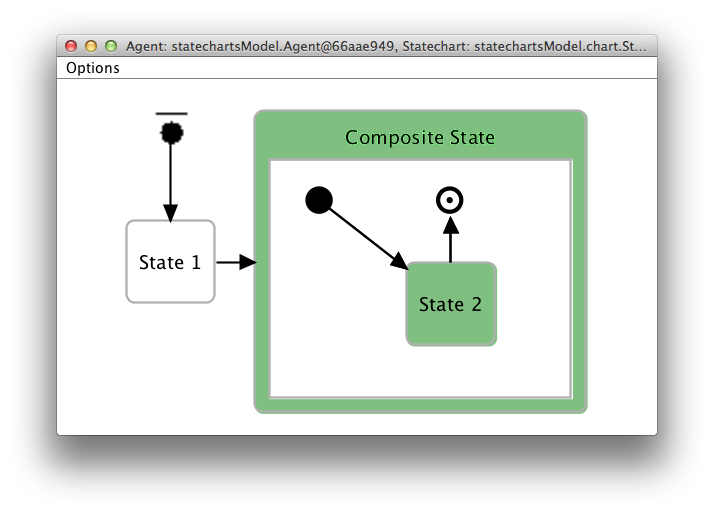
\includegraphics[width=5in]{StatechartsImages/RuntimeStatechart.png}
}
\caption{The runtime statechart display with State 2 and the Composite State that contains it highlighted as active.}
\label{fig:runtimeStatechart}
\end{center}
\end{figure}
\clearpage

\section{Putting it All Together}
In this section we provide a few simple examples for using statecharts in an agent model.

\subsection{Scheduling Agent Behavior}
Statecharts can make scheduling agent behaviors very easy to do. Figure~\ref{fig:scheduleBehaviors} shows a simple state configuration. The \emph{Go} state has a self transition with an \emph{Always} trigger and a polling time of 1 (see Figure~\ref{fig:goTrigger}) and with the \emph{On Transition} action block as shown in Figure~\ref{fig:goOnTransition}. Thus the agent will execute its \texttt{doSomething()} method at each simulation \emph{tick} until told otherwise. We can define the transition going out of the \emph{Go} state to the branching state as a \emph{Timed} transition, which will allow the agent to repeat its behavior until a certain amount of time has passed, at which point the statechart will proceed to \emph{Case 1} or \emph{Case 2} based on the condition checked by the branching state's outgoing transitions. This process can be repeated if the transitions leading back to the \emph{Go} state are followed.

\begin{figure}
\begin{center}
\vspace{.2in}
\centerline {
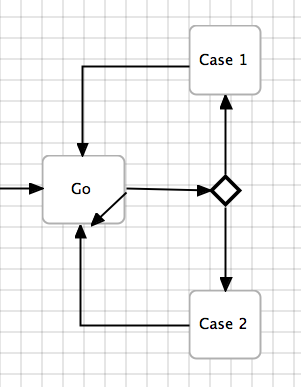
\includegraphics[width=3in]{StatechartsImages/ScheduleBehaviors.png}
}
\caption{State configuration for simple behavior scheduling.}
\label{fig:scheduleBehaviors}
\end{center}
\end{figure}


\begin{figure}
\begin{center}
\vspace{.2in}
\centerline {
\includegraphics[width=5in]{StatechartsImages/GoTrigger.png}
}
\caption{The trigger tab of the properties panel for the Go state's self transition (see Figure~\ref{fig:scheduleBehaviors}).}
\label{fig:goTrigger}
\end{center}
\end{figure}

\begin{figure}
\begin{center}
\vspace{.2in}
\centerline {
\includegraphics[width=5in]{StatechartsImages/GoOnTransition.png}
}
\caption{The \emph{On Transition} action block for the Go state's self transition (see Figure~\ref{fig:scheduleBehaviors}).}
\label{fig:goOnTransition}
\end{center}
\end{figure}

\end{document}  